In this task, we will analyze the dataset \texttt{MI\_timesteps.txt}, which contains data from the TUM Garching campus. The dataset named \texttt{MI\_timesteps.txt} covers seven weekdays and records the count of people in nine different campus areas (PID) at various times. The data, arranged in columns, is depicted in the accompanying figure (\ref{task5_1}). This time series dataset exhibits cyclical patterns, evident from multiple peaks and recurring trends.
\begin{figure}[H]
    \centering
    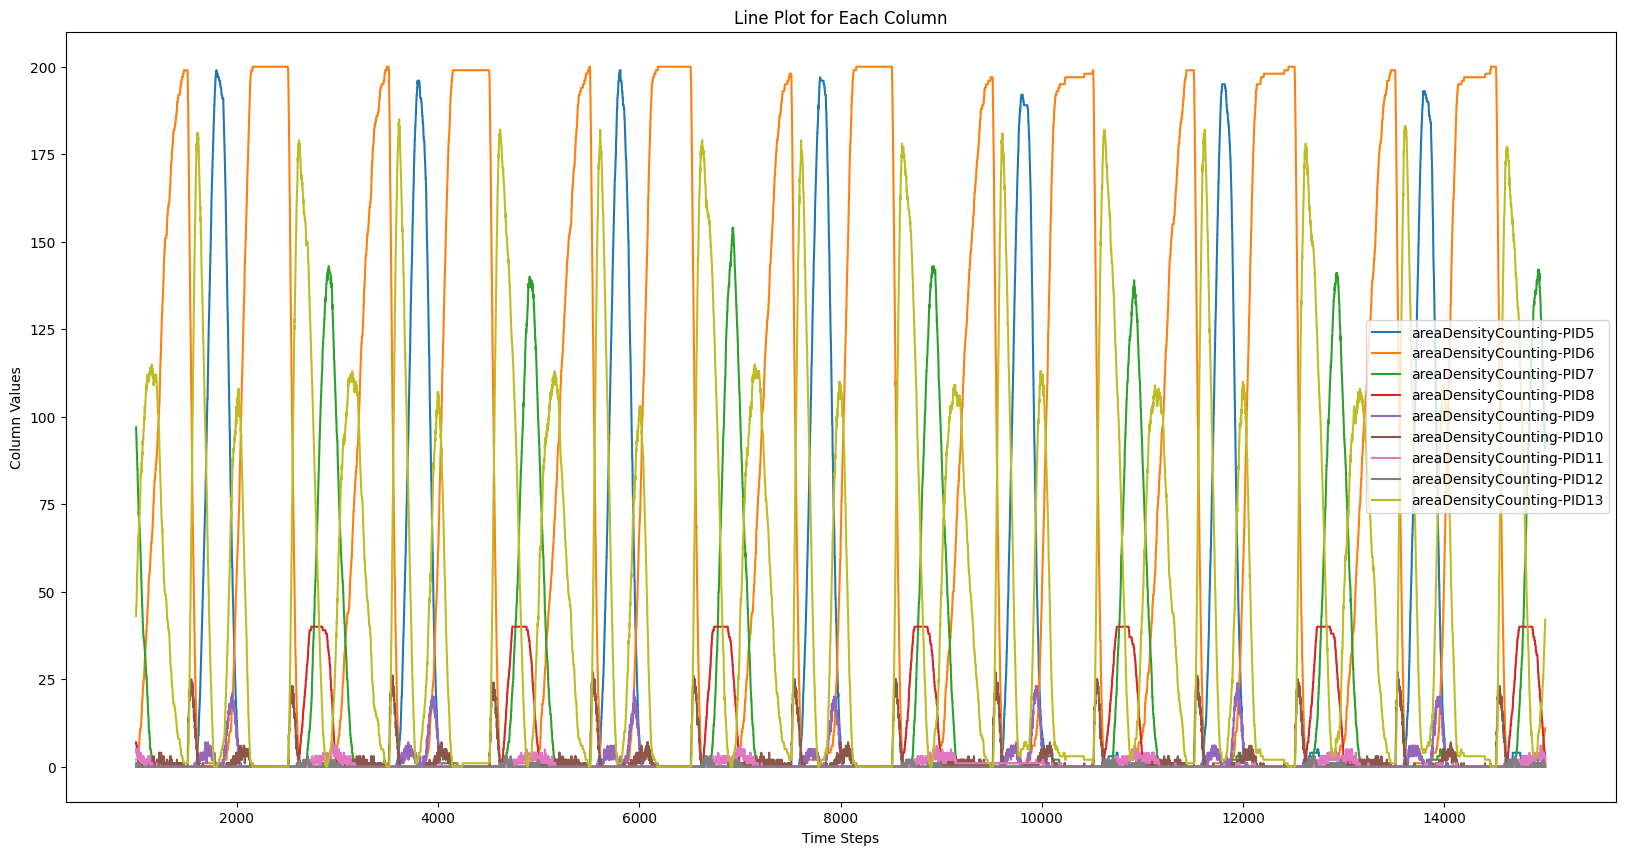
\includegraphics[width=0.8\linewidth]{images/task5_1_1.png}
    \caption{}
    \label{task5_1}
\end{figure}

Our goal is to analyze this data to predict the utilization of the MI building. We aim to learn the dynamics of the periodic curve embedded in the principal components and forecast the MI building's utilization for the upcoming 14 days. Also, the first 1000 rows of the dataset have been discarded since they are regarded as a burn-in period by the exercise sheet.\\

\begin{itemize}
    \item \textbf{Part 1: Takens theorem, delay embedding, PCA.} \\
% Part 1: How many dimensions will you need to embed the dataset according to Takens theorem? 
In Part 1, we address the task of determining the appropriate number of dimensions for embedding our dataset according to Takens' Theorem. \\

For this, we consider the dataset as a one-dimensional, periodic time series, with no apparent parametric dependencies between different time points. According to Takens' theorem, for a one-dimensional manifold, the embedding dimension required is \(2d+1\), where \(d\) is the dimensionality of the original system. Since our system is one dimensional \(d=1\), the embedding dimension needed is \(2\times 1+1=3\). However, our task specifies using windows of 351 data points across 3 measurements, resulting in vectors of 1053 dimensions. This is far above the minimum required by Takens' theorem and thus provides more detailed insights into the system's dynamics. Consequently, we will use three principal components after performing PCA. \\

% Part 1: Create a delay embedding with 350 delays of the first three measurement areas and use 3 principal components as necessary according to Takens.

In the process of creating a delay embedding with 350 delays of the first three measurement areas, we defined a function \texttt{create\_delay\_embedding} that takes the dataset and a delay parameter as inputs. This function constructs a delay embedding matrix by calculating the necessary number of rows for the embedded data, considering the specified delay. An empty matrix \texttt{embedded\_data} is initialized. The number of columns in this matrix is (delay + 1) * 3, which indicates our consideration of three columns from the original dataset for embedding. Next, a loop runs over the dataset, and for each iteration, a flattened portion of the data (spanning the current index i to i + delay + 1 and considering three columns) is added to the \texttt{embedded\_data\_matrix}. This creates a sequence of delayed observations in the dataset. After that we applied this embedding function to the data with a delay of 351, resulting in a new matrix \texttt{window\_matrix}. The shape of this matrix indicates the dimensions of the embedded data. 

\begin{figure}[H]
\centering
    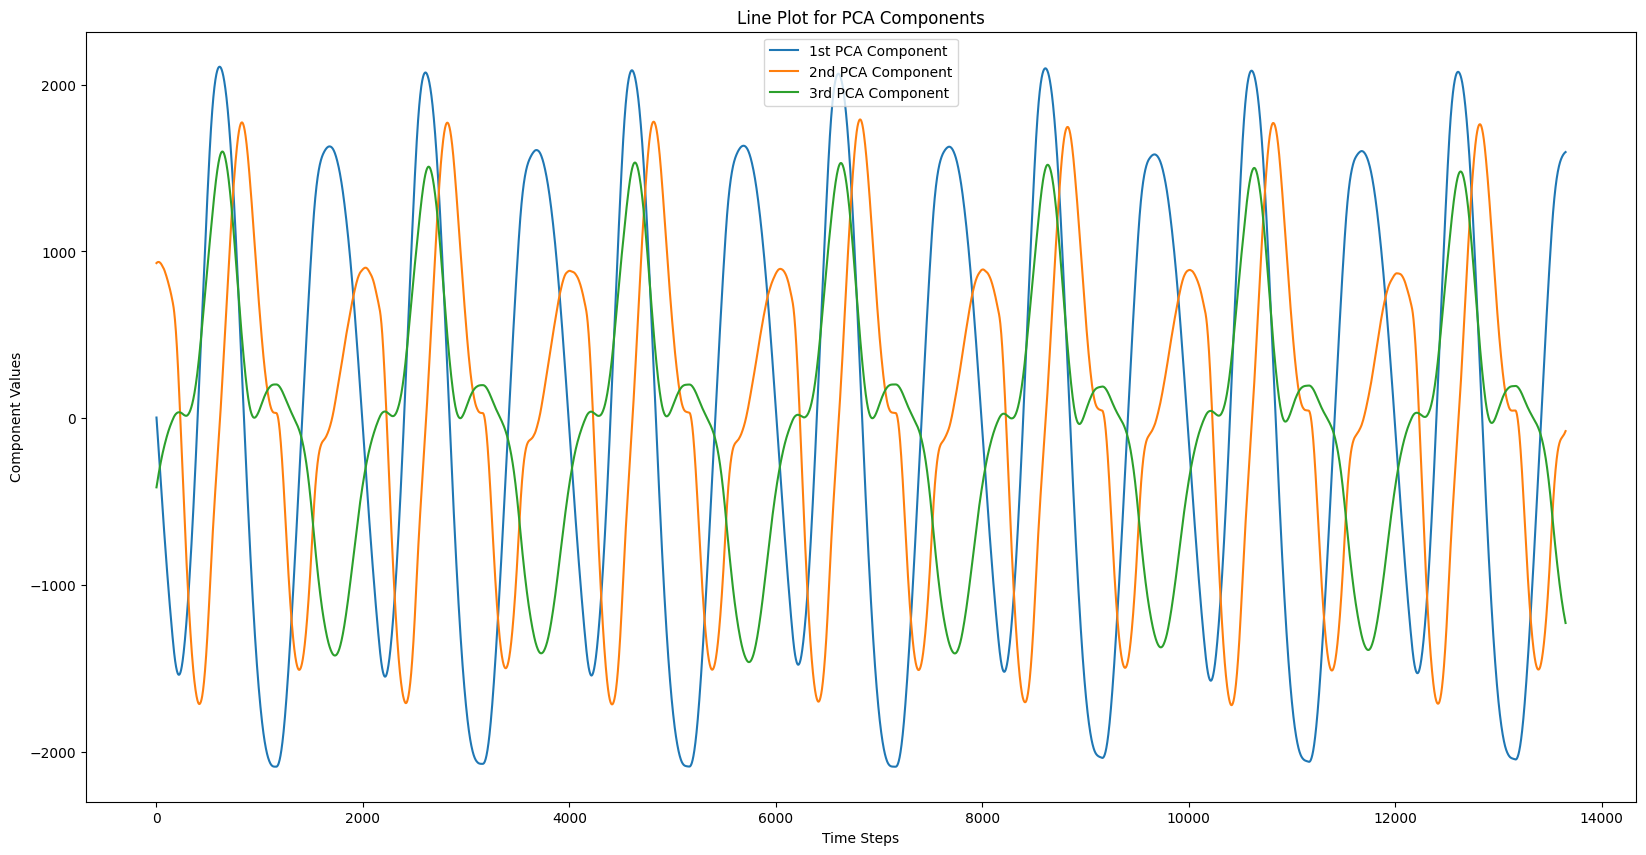
\includegraphics[width=0.8\linewidth]
    {images/task5_1_2.png}
    %\caption{}
    \label{task5_5_1_2}
\end{figure}

\begin{figure}[H]
    \centering
    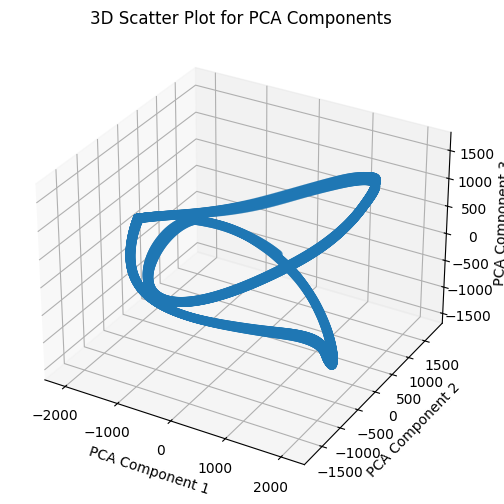
\includegraphics[width=0.5\linewidth]
    {images/task5_1_3.png}
    %\caption{}
    \label{task5_1_3}
\end{figure}

\item \textbf{Part 2:} \\
% Part 2: Color the points by the first coordinate of the delay embedding (create nine plots).
The 3D scatter plots in figure \ref{fig:task5_2} are generated by coloring the points by the first coordinate of the delay embedding. Each point on the scatter plot represents a data sample with its corresponding values on the first three principal components resulting from a PCA on the delay embedded data.

\begin{figure}[H]
\centering
    \begin{subfigure}{0.3\textwidth}
        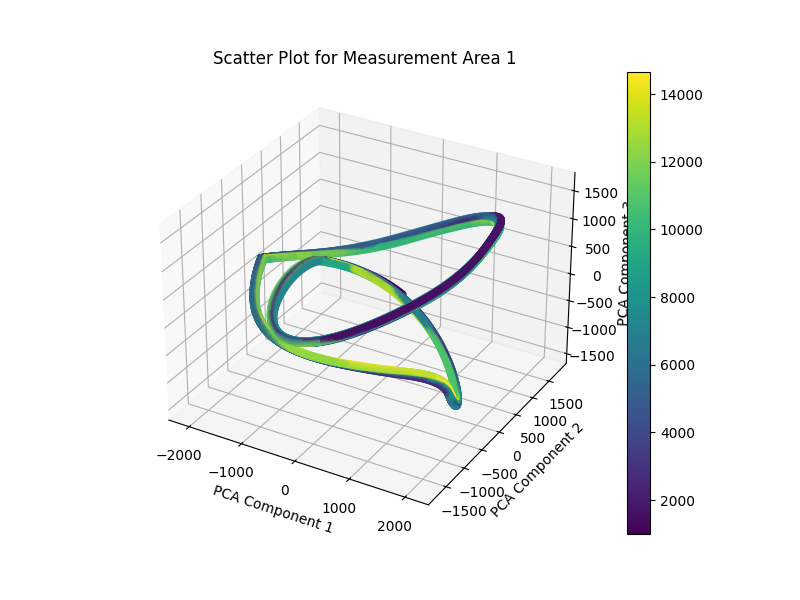
\includegraphics[width=\linewidth]
        {images/task5_2_1.png}
        \label{task5_2_1}
    \end{subfigure}
    \begin{subfigure}{0.3\textwidth}
        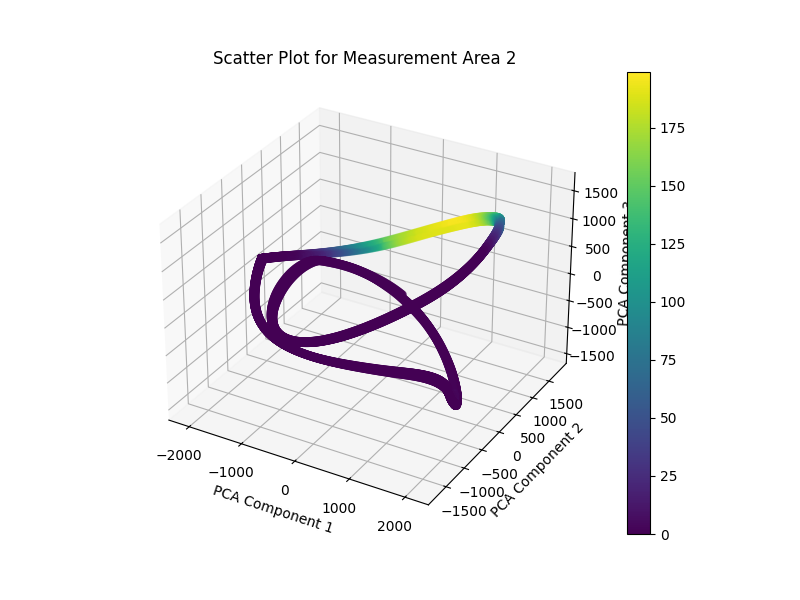
\includegraphics[width=\linewidth]
        {images/task5_2_2.png}
        \label{task5_2_2}
    \end{subfigure}
    \begin{subfigure}{0.33\textwidth}
        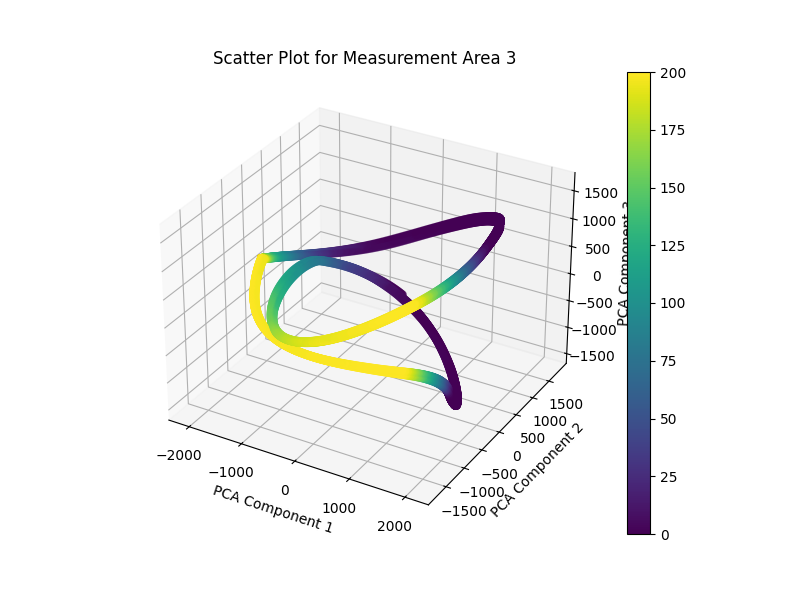
\includegraphics[width=\linewidth]
        {images/task5_2_3.png}
        \label{task5_2_3}
    \end{subfigure}
    \begin{subfigure}{0.3\textwidth}
        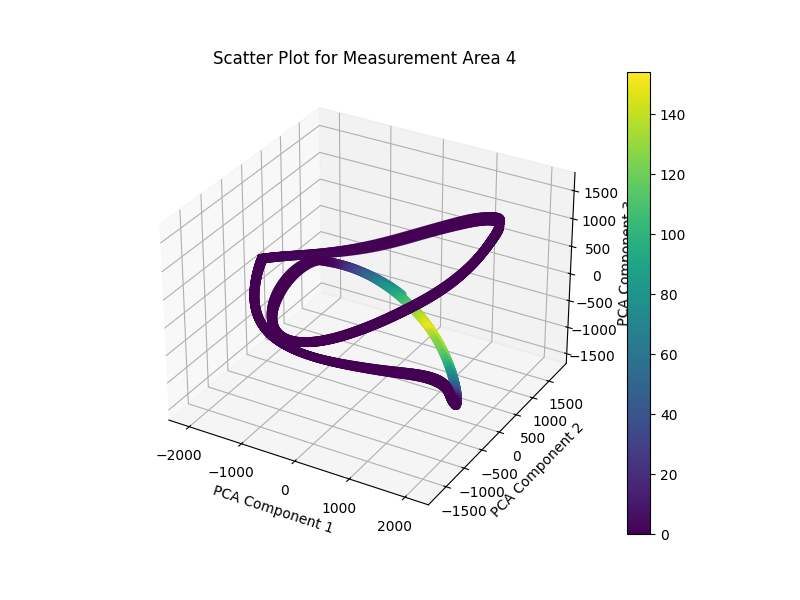
\includegraphics[width=\linewidth]
        {images/task5_2_4.png}
        \label{task5_2_4}
    \end{subfigure}
    \begin{subfigure}{0.3\textwidth}
        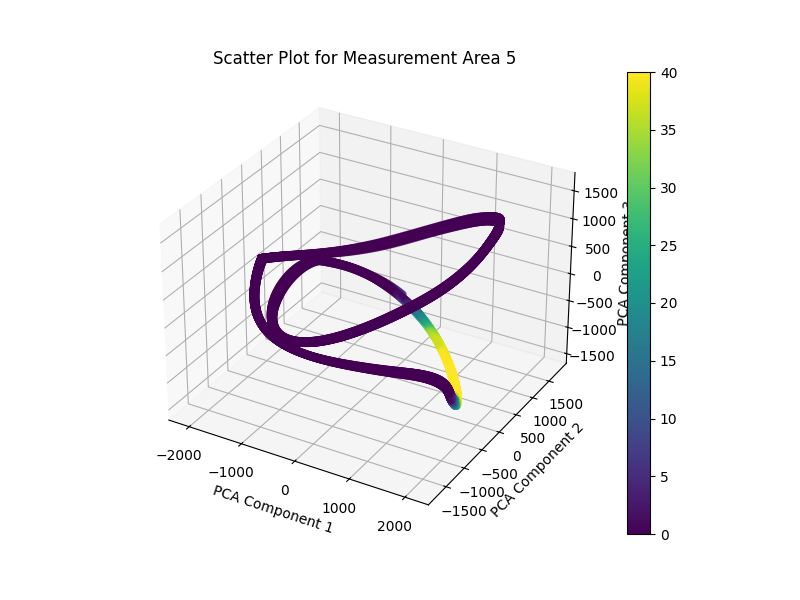
\includegraphics[width=\linewidth]
        {images/task5_2_5.png}
        \label{task5_2_5}
    \end{subfigure}
    \begin{subfigure}{0.3\textwidth}
        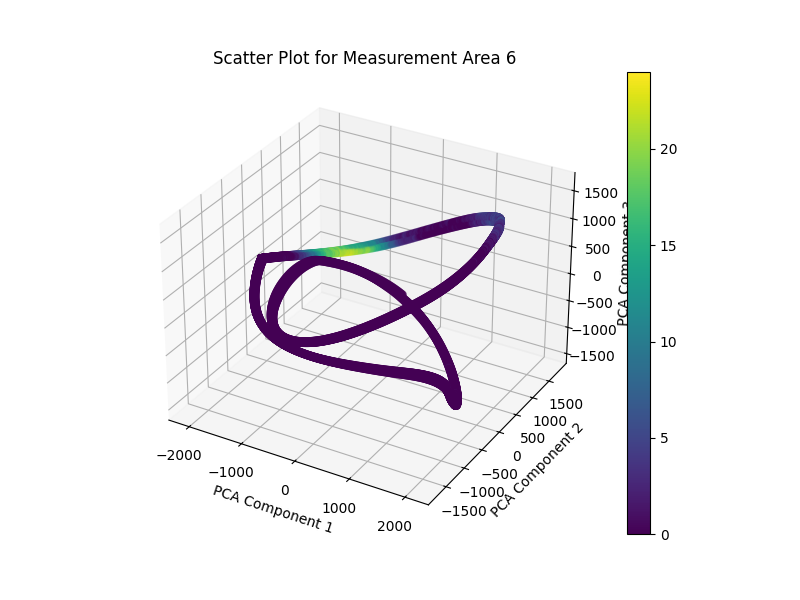
\includegraphics[width=\linewidth]
        {images/task5_2_6.png}
        \label{task5_2_6}
    \end{subfigure}
    \begin{subfigure}{0.3\textwidth}
        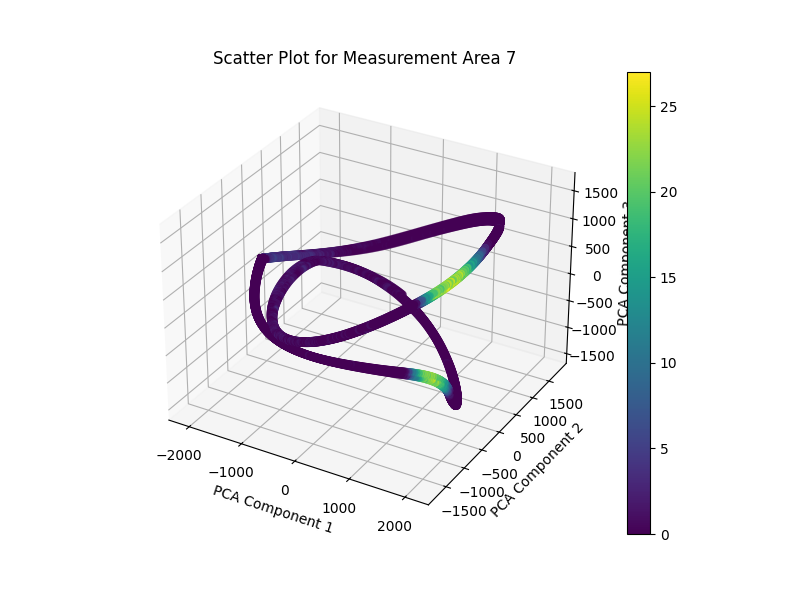
\includegraphics[width=\linewidth]
        {images/task5_2_7.png}
        \label{task5_2_7}
    \end{subfigure}
    \begin{subfigure}{0.3\textwidth}
        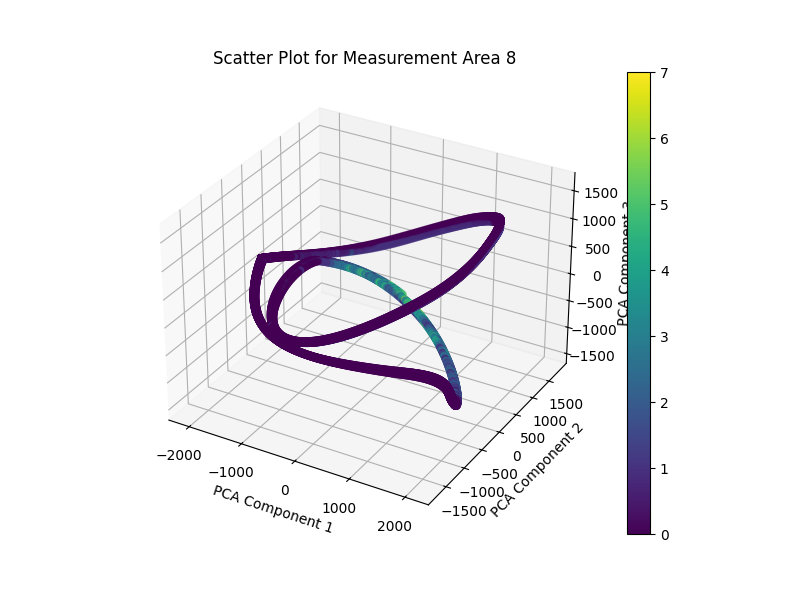
\includegraphics[width=\linewidth]
        {images/task5_2_8.png}
        \label{task5_2_8}
    \end{subfigure}
    \begin{subfigure}{0.3\textwidth}
        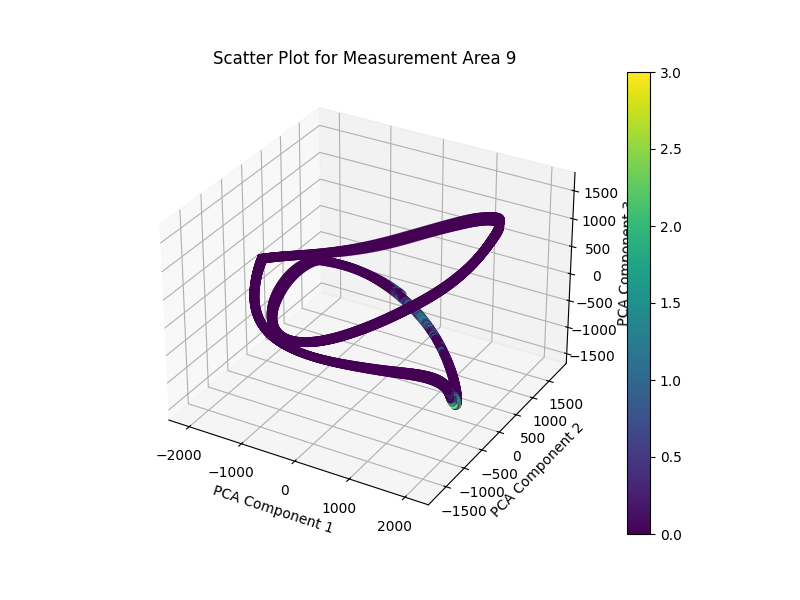
\includegraphics[width=\linewidth]
        {images/task5_2_9.png}
        \label{task5_2_9}
    \end{subfigure}
    \caption{}
    \label{fig:task5_2}
\end{figure}

PCA is employed to capture the most significant patterns in the dataset by reducing its dimensionality. The three axes—PCA Component 1, PCA Component 2, and PCA Component 3—represent the directions with the highest variance in the data, which are crucial to understanding the dynamics of campus utilization. We can observe that all the points are in the same position only the color changes, The color scale in each plot corresponds to the first coordinate of the delay embedding, which is indicative of the sequential time at which the data was recorded. The gradation of colors provides insights into the temporal progression of the density count.

 
\item \textbf{Part 3:} \\
For this task, we have to learn the dynamics of the periodic curve that we already embedded in the principal components of the previous task. For this, we first extract the time steps present in the first column of the dataset. Then we calculate the distances between consecutive points (\texttt{deltas}) of the PCA space and use \texttt{np.linalg.norm} over the found deltas to compute the arclengths. We store the cumulative sum at each point using the \texttt{np.cumsum} method.\\
Then, we calculate velocities or the rate of change of arclengths over time. We plot this velocity vs the cumulative arclength as seen in figure \ref{fig:task5_3_1}. The periodic nature of the dataset becomes apparent in this plot. To gain a more detailed understanding, we can trim one complete period of the data and visualize it separately, as illustrated in figure \ref{task5_3_2}.
\begin{figure}[H]
\centering
    \begin{subfigure}{0.45\textwidth}
        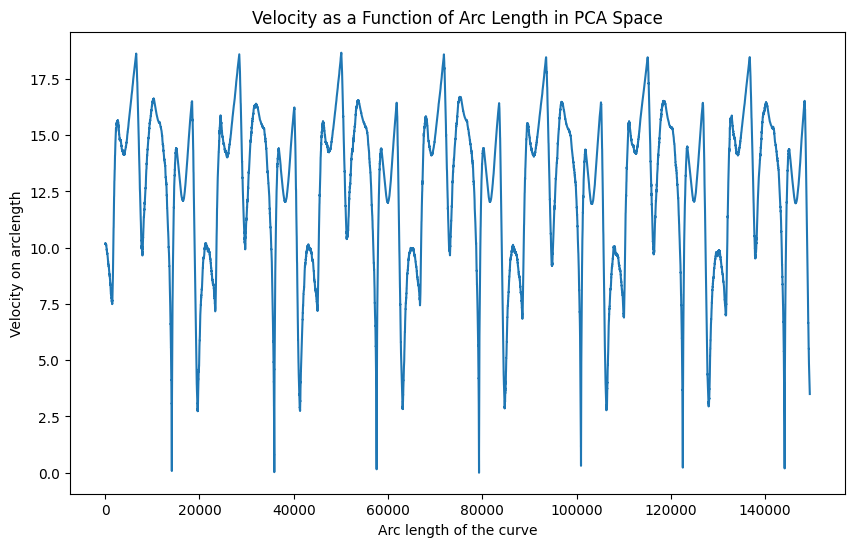
\includegraphics[width=\linewidth]{images/Ex5task5_31.png}
        \caption{Plot for the entire dataset}
        \label{fig:task5_3_1}
    \end{subfigure}
    \begin{subfigure}{0.45\textwidth}
        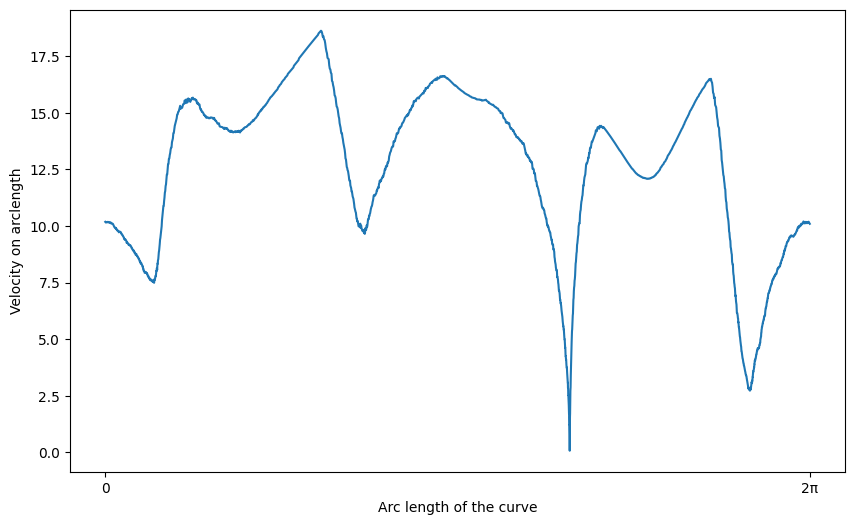
\includegraphics[width=\linewidth]
        {images/Ex5task5_32.png}
        \caption{Plot for one period}
        \label{task5_3_2}
    \end{subfigure}
    \label{task5_3}
    \caption{}
\end{figure}

\item \textbf{Part 4:}\\
For this final task, we had to predict the utilization of the MI building for the next 14 days. To do this, we used the periodic feature of the dataset and extrapolated our calculated velocities to a period of 14 days. This extension enabled us to understand the system's dynamics over a more prolonged timeframe.\\
We then need to calculate the arclength over this period of 14 days. To do this, we calculated the cumulative sum of the extrapolated velocities and extended time intervals embedded within the principal component. This allowed us to project the system's behaviours over a period of 14 days. Now, to model the relationship between arclength and the measurement parameter, we utilized the radial basis function (RBF) approximation implemented in task 1. The least square minimization technique was used to derive optimal coefficients for the RBF model. The final predicted vs original plot can be seen in figure \ref{fig:task5_4_final}.


\begin{figure}[H]
    \centering
    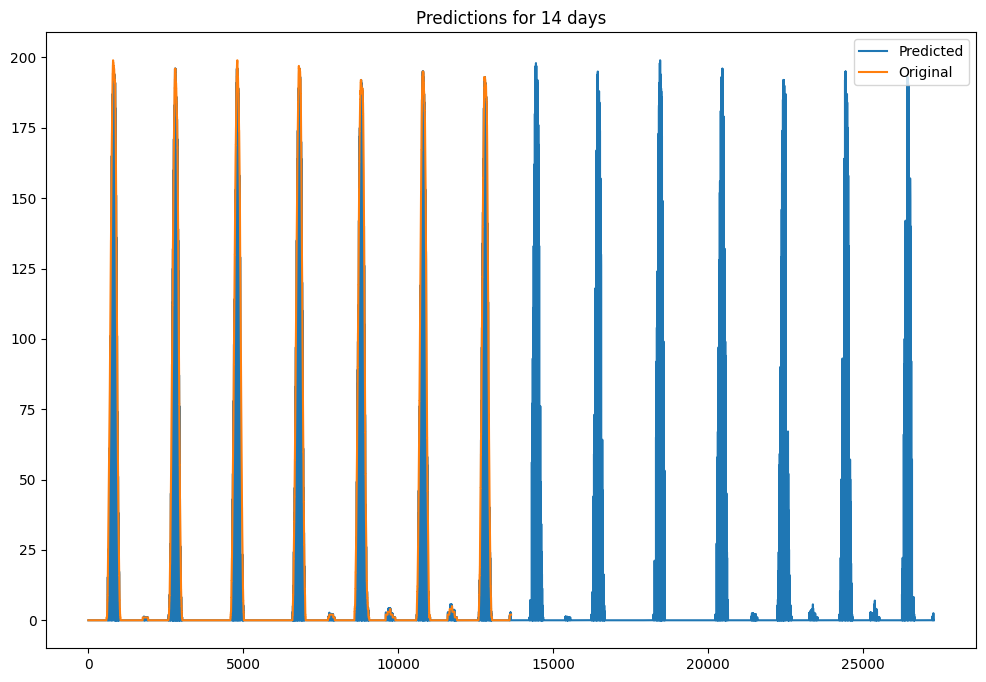
\includegraphics[width=0.9\linewidth]{images/Ex5task5_42.png}
    \caption{Predictions for 14 days}
    \label{fig:task5_4_final}
\end{figure}

% Part 3: Learn the dynamics on the periodic curve you embedded in the principal components.
% Part 3: Predict the utilization of the MI building for the next 14 days...
% Part 3: ... which should look like one of the graphs in figure 3, just about twice as long.

% Discussed how and why you chose the values of L and ϵ?


\end{itemize}